\chapter{Régimes transitoires~: premier et second ordre}\label{ch:b1:transient-regimes}

Appuyez sur le coin d'une voiture à l'arrêt, puis lâchez. Une voiture en
bon état remonte une fois et s'arrête~; une voiture aux amortisseurs
fatigués oscille deux ou trois fois avant de se stabiliser. Dans un
laboratoire d'électronique, les deux mêmes comportements apparaissent à
l'oscilloscope lorsqu'un condensateur se décharge dans une bobine~: un
retour sans oscillation, ou une sonnerie qui s'éteint. L'un et l'autre
sont le \emph{transitoire} entre deux \omterm{def:b1:transient-regimes:firstorder}{régimes permanents}, et tous deux
obéissent à la même petite famille d'équations différentielles linéaires
--- du premier ordre pour un seul réservoir d'énergie, du second ordre
pour deux qui s'échangent. Ce chapitre les résout une fois pour toutes,
nomme leurs paramètres (\omterm{def:b1:transient-regimes:firstorder}{constante de temps}, \omterm{def:b1:transient-regimes:secondorder}{pulsation propre}, \omterm{def:b1:transient-regimes:secondorder}{facteur de
qualité}), et montre que les mêmes nombres décrivent un circuit et une
suspension.

\begin{omfigure}
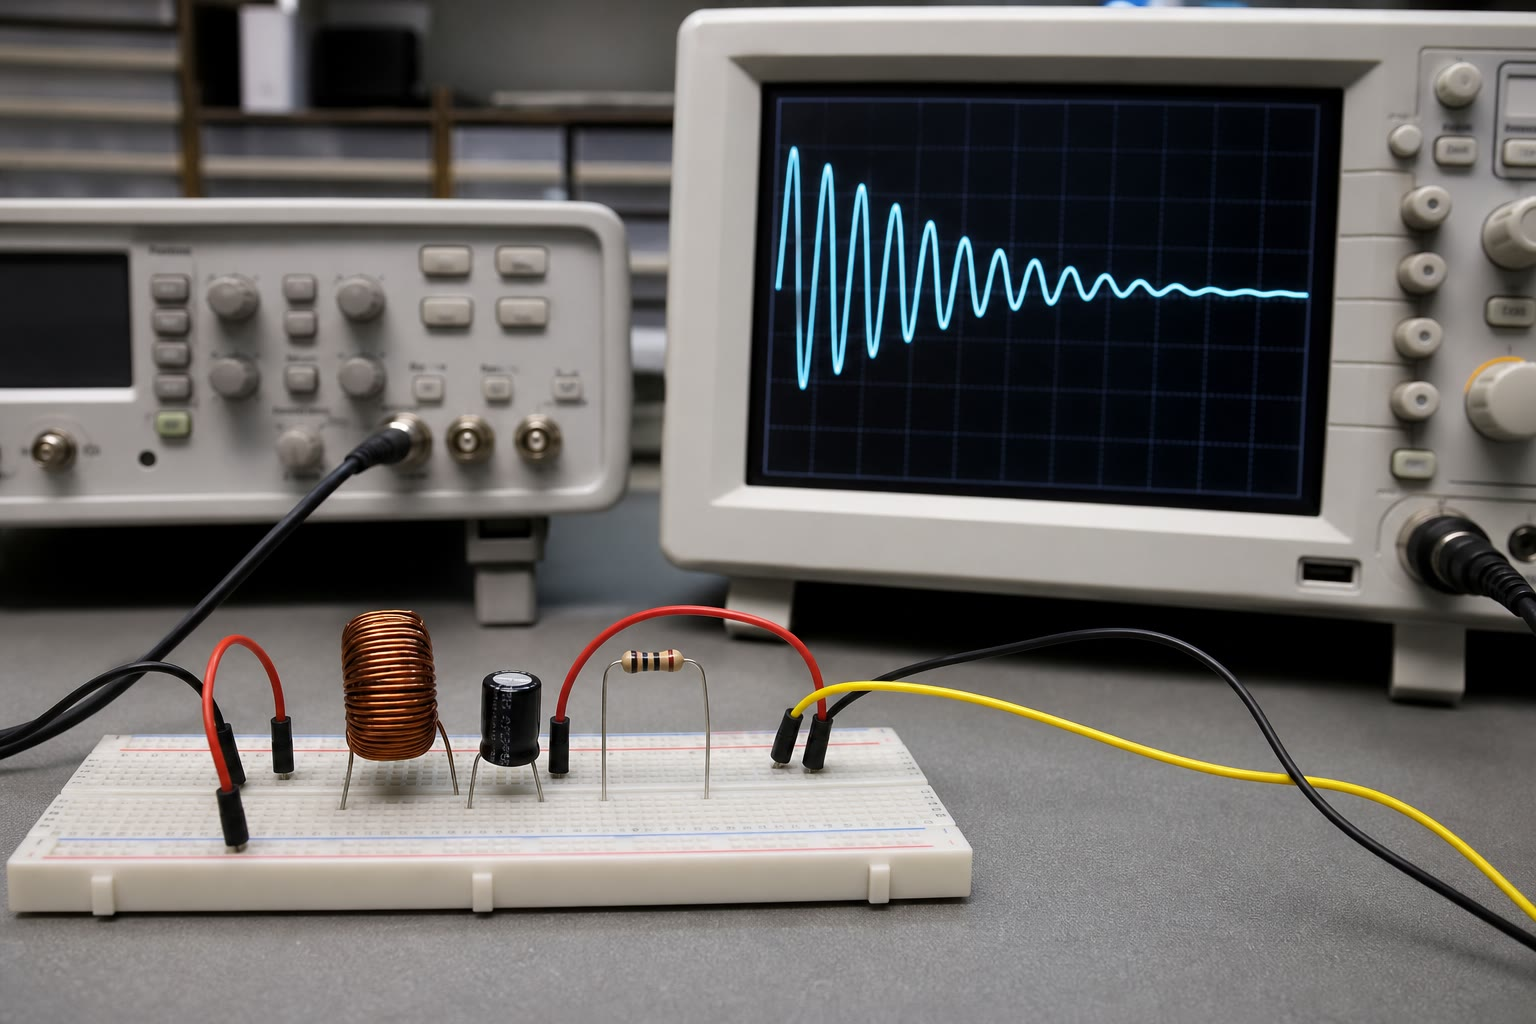
\includegraphics[width=0.60\linewidth]{images/book3/ai/b3-07-rlc-breadboard-oscilloscope.jpg}

{\small Une bobine, un condensateur et une résistance sur une plaque d'essai, et à l'oscilloscope l'oscillation amortie qui suit un échelon~: le \omterm{thm:b1:transient-regimes:regimes}{régime pseudo-périodique} de ce chapitre.}
\end{omfigure}

\section{Systèmes du premier ordre}

\begin{definition}[Système linéaire du premier ordre]\label{def:b1:transient-regimes:firstorder}
\index{système du premier ordre}\index{constante de temps}\index{régime transitoire}\index{régime permanent}
Une grandeur $x(t)$ obéit à une \emph{équation linéaire du premier ordre
à coefficients constants} lorsque
\[
\tau\,\frac{\dd x}{\dd t} + x = x_\infty ,
\]
avec $\tau > 0$ la \emph{constante de temps} et $x_\infty$ une constante
(la valeur imposée par la source). Son \emph{régime permanent} est
$x = x_\infty$~; le \emph{régime transitoire} est l'approche vers lui
depuis la valeur initiale $x(0) = x_0$.
\end{definition}

\begin{theorem}[Solution]\label{thm:b1:transient-regimes:firstorder}
L'unique solution vérifiant $x(0) = x_0$ est
\[
x(t) = x_\infty + (x_0 - x_\infty)\,\eu^{-t/\tau} .
\]
L'écart au \omterm{def:b1:transient-regimes:firstorder}{régime permanent} est divisé par $\eu^{-1} \approx
0.37$ à chaque $\tau$~: $63\%$ du chemin en $\tau$, $95\%$ en $3\tau$,
$99\%$ en $4.6\tau$. La tangente à l'origine atteint $x_\infty$ en
$t = \tau$.
\end{theorem}

\begin{proof}
$y = x - x_\infty$ obéit à $\tau y' + y = 0$, dont les solutions sont
$y = K\eu^{-t/\tau}$ (le cours de mathématiques sur les équations
différentielles linéaires démontre qu'il n'y en a pas d'autres)~;
$K = x_0 - x_\infty$. La pente en $0$ vaut $-(x_0 - x_\infty)/\tau$, qui
comblerait l'écart en une durée $\tau$.
\end{proof}

\begin{omfigure}
\begin{tikzpicture}
\begin{axis}[omaxis, width=9.4cm, height=5.4cm, xlabel={$t$}, ylabel={$x$},
    xmin=0, xmax=5, ymin=0, ymax=1.35, xtick={1,2,3,4,5},
    xticklabels={$\tau$,$2\tau$,$3\tau$,$4\tau$,$5\tau$},
    ytick={0.632,1}, yticklabels={$0.63$,$x_\infty$}]
  \addplot[omExo, dashed, domain=0:5, samples=2] {1};
  \addplot[omExo, dashed, domain=0:1, samples=2] {x};
  \addplot[omDef, thick, domain=0:5, samples=100] {1 - exp(-x)};
  \draw[dashed, omExo] (axis cs:1,0) -- (axis cs:1,0.632) -- (axis cs:0,0.632);
  \draw[dashed, omExo] (axis cs:3,0) -- (axis cs:3,0.95);
  \node[omExo, below right, font=\footnotesize] at (axis cs:3,0.95) {$0.95\,x_\infty$};
  \node[omDef, font=\footnotesize, below right] at (axis cs:2.2,0.75) {$x_\infty(1 - \eu^{-t/\tau})$};
\end{axis}
\end{tikzpicture}

{\small Réponse indicielle du premier ordre depuis $x_0 = 0$~: la
tangente initiale rencontre l'asymptote en $t = \tau$~; $63\%$ du chemin
en $\tau$, $95\%$ en $3\tau$. Tout transitoire du premier ordre est
cette courbe, dilatée par $\tau$ et translatée par $x_0$ et $x_\infty$.}
\end{omfigure}

\begin{proposition}[Circuits RC et RL]\label{prop:b1:transient-regimes:rcrl}
\index{circuit RC}\index{circuit RL}
Un condensateur $C$ chargé à travers une résistance $R$ par une source
idéale $E$ obéit à $RC\,\dd u_C/\dd t + u_C = E$~: $\tau = RC$,
$u_{C,\infty} = E$. Une bobine $L$ en série avec $R$ sous $E$ obéit à $(L/R)\,\dd i/\dd t + i =
E/R$~: $\tau = L/R$, $i_\infty = E/R$. Source retirée
($E \to 0$), les mêmes équations décrivent la décharge vers zéro.
\end{proposition}

\begin{proof}
\omterm{thm:b1:dc-circuits:kirchhoff}{Loi des mailles} $E = Ri + u_C$ avec $i = C\,\dd u_C/\dd t$~; \omterm{thm:b1:dc-circuits:kirchhoff}{loi des
mailles} $E = Ri + L\,\dd i/\dd t$.
\end{proof}

\begin{proposition}[Conditions de continuité]\label{prop:b1:transient-regimes:continuity}
\index{continuité (de $u_C$, de $i_L$)}
La tension aux bornes d'un condensateur et le courant dans une bobine
sont des fonctions continues du temps~: à un instant de commutation
$t_0$, $u_C(t_0^+) = u_C(t_0^-)$ et $i_L(t_0^+) = i_L(t_0^-)$. Les
courants dans les résistances et les tensions aux bornes des bobines
peuvent, elles, sauter.
\end{proposition}

\begin{proof}
Un saut de $u_C$ exigerait $i = C\,\dd u_C/\dd t$ infini, un saut de
$i_L$ exigerait $u = L\,\dd i/\dd t$ infini~; l'un et l'autre sont
impossibles dans un circuit aux tensions et courants finis (de façon
équivalente, les énergies stockées $\tfrac12 Cu_C^2$ et $\tfrac12 Li^2$
ne peuvent varier instantanément sans puissance infinie).
\end{proof}

\begin{method}[Résoudre un transitoire du premier ordre]\label{met:b1:transient-regimes:first}
\begin{enumerate}
  \item Écrire les \omterm{thm:b1:dc-circuits:kirchhoff}{lois des mailles} et des nœuds après la commutation,
        avec les lois des composants~; se ramener à une seule équation
        en $u_C$ ou $i_L$ et la mettre sous la forme
        $\tau x' + x = x_\infty$~; y lire $\tau$ et $x_\infty$ (cette
        dernière est aussi le \omterm{def:b1:transient-regimes:firstorder}{régime permanent}, obtenu en remplaçant $C$
        par un circuit ouvert et $L$ par un fil).
  \item Trouver $x_0$ par continuité de $u_C$ ou de $i_L$ à l'instant de
        commutation, en utilisant le circuit \emph{d'avant}.
  \item Écrire $x = x_\infty + (x_0 - x_\infty)\eu^{-t/\tau}$~; en
        déduire les autres grandeurs par dérivation et \omterm{thm:b1:dc-circuits:kirchhoff}{loi des mailles}.
\end{enumerate}
Lorsque le condensateur voit un réseau de résistances et de sources, on
remplace d'abord ce réseau par son équivalent de Thévenin
$(E_{\mathrm{Th}}, R_{\mathrm{Th}})$
(\cref{ch:b1:dc-circuits})~: $\tau = R_{\mathrm{Th}}C$,
$u_\infty = E_{\mathrm{Th}}$.
\end{method}

\begin{proposition}[Bilan énergétique de la charge d'un RC]\label{prop:b1:transient-regimes:rcenergy}
En chargeant un condensateur de $0$ à $E$ à travers une résistance $R$
quelconque, la source fournit $CE^2$, le condensateur stocke
$\tfrac12 CE^2$, et la résistance dissipe l'autre $\tfrac12 CE^2$ ---
quelle que soit $R$.
\end{proposition}

\begin{proof}
$i = (E/R)\eu^{-t/\tau}$~; la source fournit $\int_0^\infty Ei\,\dd t
= E \cdot (E/R)\tau = CE^2$~; la résistance prend $\int_0^\infty Ri^2\,\dd t
= (E^2/R)\int_0^\infty \eu^{-2t/\tau}\dd t = (E^2/R)(\tau/2) = \tfrac12 CE^2$~;
la différence est l'énergie stockée $\tfrac12 CE^2$. Une $R$ plus petite
dissipe la même énergie plus vite.
\end{proof}

\begin{example}[La bobine d'un relais]\label{ex:b1:transient-regimes:relay}
$L = \qty{20}{mH}$, $R = \qty{5.0}{\ohm}$, $E = \qty{10}{V}$~: $\tau =
\qty{4.0}{ms}$, $i_\infty = \qty{2.0}{A}$~; les contacts se ferment
lorsque $i$ atteint \qty{1.5}{A}, c'est-à-dire en $t = -\tau\ln(1 - 0.75) =
\qty{5.5}{ms}$. À l'ouverture du circuit, $i$ doit retomber depuis
\qty{2}{A}~; une diode «~de roue libre~» placée aux bornes de la bobine
lui offre un chemin par $R$ seule, $\tau = \qty{4}{ms}$, au lieu d'une
étincelle.
\end{example}

\section{Systèmes du second ordre}

\begin{definition}[Forme canonique du second ordre]\label{def:b1:transient-regimes:secondorder}
\index{système du second ordre}\index{pulsation propre}\index{facteur de qualité}\index{coefficient d'amortissement}
Une grandeur $x(t)$ est un \emph{système linéaire du second ordre} lorsque
\[
\frac{\dd^2 x}{\dd t^2} + \frac{\omega_0}{Q}\,\frac{\dd x}{\dd t} + \omega_0^2\,x
= \omega_0^2\,x_\infty ,
\]
avec $\omega_0 > 0$ la \emph{\omterm{def:b1:wave-propagation:signal}{pulsation} propre}, $Q > 0$ le \emph{facteur
de qualité} (\omterm{def:b1:units-dimensions:dimension}{sans dimension}), et $x_\infty$ le \omterm{def:b1:transient-regimes:firstorder}{régime permanent}. On
écrit aussi $\omega_0/Q = 2\xi\omega_0$, avec $\xi = 1/2Q$ le
\emph{coefficient d'amortissement}.
\end{definition}

\begin{proposition}[Le circuit RLC série]\label{prop:b1:transient-regimes:rlc}
\index{circuit RLC}
Un condensateur $C$, une bobine $L$ et une résistance $R$ en série sous
une source $E$~: la tension du condensateur obéit à la forme canonique avec
\[
\omega_0 = \frac{1}{\sqrt{LC}}, \qquad Q = \frac{1}{R}\sqrt{\frac{L}{C}},
\qquad u_{C,\infty} = E .
\]
\end{proposition}

\begin{proof}
\omterm{thm:b1:dc-circuits:kirchhoff}{Loi des mailles}~: $E = L\,\dd i/\dd t + Ri + u_C$ avec $i = C\,\dd u_C/\dd t$~:
$LC\,u_C'' + RC\,u_C' + u_C = E$~; on divise par $LC$ et on identifie
$\omega_0^2 = 1/LC$, $\omega_0/Q = R/L$.
\end{proof}

\begin{omfigure}
\begin{tikzpicture}[font=\small]
  \draw (0,0) to[battery1, l=$E$, invert] (0,2.6) to[R=$R$] (2.4,2.6) to[L=$L$, i=$i$] (4.8,2.6) -- (4.8,2.6) to[C=$C$, v=$u_C$] (4.8,0) -- (0,0);
  \begin{scope}[xshift=7.6cm]
    \draw[thick] (0,0) -- (0,3.4);
    \fill[pattern=north east lines] (-0.25,0) rectangle (0,3.4);
    % spring
    \draw[thick] (0,2.6) -- (0.4,2.6) \foreach \i in {0,...,5} {-- ++(0.2,0.25) -- ++(0.2,-0.5) -- ++(0.2,0.25)} -- (3.3,2.6);
    % damper
    \draw[thick] (0,0.8) -- (1.2,0.8);
    \draw[thick] (1.2,0.5) -- (1.2,1.1) -- (2.2,1.1); \draw[thick] (1.2,0.5) -- (2.2,0.5);
    \draw[thick] (1.9,0.6) -- (1.9,1.0); \draw[thick] (1.9,0.8) -- (3.3,0.8);
    \draw[thick, fill=omDef!15] (3.3,0.2) rectangle (4.5,3.2); \node at (3.9,1.7) {$m$};
    \draw[-Stealth] (3.9,3.5) -- (5.2,3.5) node[right] {$x$};
    \node at (1.7,3.15) {$k$}; \node at (1.7,0.1) {$\alpha$};
  \end{scope}
\end{tikzpicture}

{\small Les deux visages du \omterm{def:b1:transient-regimes:secondorder}{système du second ordre}~: le \omterm{prop:b1:transient-regimes:rlc}{circuit RLC}
série ($\omega_0 = 1/\sqrt{LC}$, $Q = \sqrt{L/C}/R$) et le système
masse--ressort--amortisseur ($\omega_0 = \sqrt{k/m}$,
$Q = \sqrt{km}/\alpha$). Même équation, mêmes trois régimes.}
\end{omfigure}

\begin{proposition}[L'oscillateur mécanique]\label{prop:b1:transient-regimes:mechanical}
\index{masse--ressort--amortisseur}\index{analogie électromécanique}
Une masse $m$ au bout d'un ressort de raideur $k$, munie d'un
amortisseur visqueux de coefficient $\alpha$ (force $-\alpha\dot x$), et
écartée de $x$ de sa position d'équilibre, obéit à
$m\ddot x + \alpha\dot x + kx = 0$~: c'est la forme canonique avec
\[
\omega_0 = \sqrt{\frac{k}{m}}, \qquad Q = \frac{\sqrt{km}}{\alpha} .
\]
La correspondance $x \leftrightarrow q$, $\dot x \leftrightarrow i$,
$m \leftrightarrow L$, $\alpha \leftrightarrow R$, $k \leftrightarrow 1/C$
transporte tout résultat d'un système sur l'autre.
\end{proposition}

\begin{proof}
La deuxième loi de Newton (\cref{ch:b1:newton-dynamics}) avec la force
de rappel $-kx$ et la force d'amortissement~; on divise par $m$.
\end{proof}

\begin{theorem}[Les trois régimes]\label{thm:b1:transient-regimes:regimes}
\index{régime apériodique}\index{régime critique}\index{régime pseudo-périodique}\index{pseudo-période}
Les solutions de l'équation homogène $x'' + (\omega_0/Q)x' +
\omega_0^2 x = 0$ sont gouvernées par les racines de $r^2 + (\omega_0/Q)r +
\omega_0^2 = 0$, de discriminant $\Delta = \omega_0^2(1/Q^2 - 4)$~:
\begin{itemize}
  \item $Q < \tfrac12$, régime \emph{apériodique}~: deux racines réelles
        négatives $r_\pm = -\frac{\omega_0}{2Q}\big(1 \mp \sqrt{1 - 4Q^2}\big)$,
        $x = A\eu^{r_+t} + B\eu^{r_-t}$, un retour sans oscillation~;
  \item $Q = \tfrac12$, régime \emph{critique}~: une racine double
        $r = -\omega_0$, $x = (A + Bt)\eu^{-\omega_0 t}$, le retour le
        plus rapide sans dépassement~;
  \item $Q > \tfrac12$, régime \emph{pseudo-périodique}~: racines
        complexes $r = -1/\tau \pm \iu\omega$ avec
        \[
        \tau = \frac{2Q}{\omega_0}, \qquad
        \omega = \omega_0\sqrt{1 - \frac{1}{4Q^2}},
        \qquad
        x = \eu^{-t/\tau}\big(A\cos\omega t + B\sin\omega t\big),
        \]
        une oscillation amortie de \emph{pseudo-période} $T = 2\pi/\omega$
        à l'intérieur de l'enveloppe $\pm\sqrt{A^2 + B^2}\,\eu^{-t/\tau}$.
\end{itemize}
La solution complète avec un second membre constant est $x_\infty$ plus
la solution homogène~; $A$ et $B$ se tirent de $x(0)$ et $x'(0)$.
\end{theorem}

\begin{proof}
Équation caractéristique d'une équation linéaire à coefficients
constants (cours de mathématiques, équations linéaires du second
ordre)~: les racines valent $r = -\omega_0/2Q \pm \tfrac12\sqrt\Delta$. Pour $Q > \tfrac12$,
$\sqrt\Delta = \iu\omega_0\sqrt{4 - 1/Q^2}$, d'où la partie réelle
$-\omega_0/2Q = -1/\tau$ et la partie imaginaire $\pm\omega_0\sqrt{1 - 1/4Q^2}$~;
les solutions réelles sont les combinaisons de $\eu^{-t/\tau}\cos\omega t$
et de $\eu^{-t/\tau}\sin\omega t$.
\end{proof}

\begin{omfigure}
\begin{tikzpicture}
\begin{axis}[omaxis, width=11.5cm, height=6cm, xlabel={$\omega_0 t$}, ylabel={$x/x_\infty$},
    xmin=0, xmax=16, ymin=0, ymax=1.75, xtick={0,5,10,15}, ytick={0.5,1,1.5},
    legend style={at={(0.97,0.97)}, anchor=north east, font=\footnotesize, draw=none, fill=none}]
  % Q=0.2: roots r = -(1/(2Q))(1 -/+ sqrt(1-4Q^2)) = -2.5(1 -/+ 0.6) = -1, -4 ; x = 1 - (4 e^{-t} - e^{-4t})/3
  \addplot[omProp, thick, domain=0:16, samples=200] {1 - (4*exp(-x) - exp(-4*x))/3};
  \addlegendentry{$Q = 0.2$ (apériodique)}
  \addplot[omThm, thick, domain=0:16, samples=200] {1 - (1 + x)*exp(-x)};
  \addlegendentry{$Q = 0.5$ (critique)}
  % Q=3: tau=6, w = sqrt(1-1/36)=0.986 ; x = 1 - e^{-t/6}(cos wt + sin wt /(6 w))
  \addplot[omDef, thick, domain=0:16, samples=400] {1 - exp(-x/6)*(cos(deg(0.986*x)) + sin(deg(0.986*x))/(6*0.986))};
  \addlegendentry{$Q = 3$ (pseudo-périodique)}
  \addplot[omExo, dashed, domain=0:16, samples=2] {1};
\end{axis}
\end{tikzpicture}

{\small Réponse indicielle d'un \omterm{def:b1:transient-regimes:secondorder}{système du second ordre} initialement au
repos, pour trois \omterm{def:b1:transient-regimes:secondorder}{facteurs de qualité}. $Q$ petit~: une reptation lente~;
$Q = \tfrac12$~: le retour le plus rapide sans dépassement~; $Q$ grand~:
une sonnerie qui dure environ $Q$ oscillations.}
\end{omfigure}

\begin{proposition}[Lire $Q$ sur un tracé pseudo-périodique]\label{prop:b1:transient-regimes:decrement}
\index{décrément logarithmique}
En \omterm{thm:b1:transient-regimes:regimes}{régime pseudo-périodique}, deux maxima successifs sont dans le rapport
$x_{n+1}/x_n = \eu^{-T/\tau}$~; le \emph{\omterm{prop:b1:transient-regimes:decrement}{décrément logarithmique}}
\[
\delta = \ln\frac{x_n}{x_{n+1}} = \frac{T}{\tau} = \frac{\pi}{Q\sqrt{1 - 1/4Q^2}}
\approx \frac{\pi}{Q} \quad (Q \gg 1)
\]
donne $Q$~; le nombre d'oscillations visibles avant que l'\omterm{def:b1:wave-propagation:signal}{amplitude} ne
tombe sous $5\%$ vaut environ $Q$. Pour $Q \gg 1$, $\omega \approx \omega_0$
et $T \approx 2\pi/\omega_0$.
\end{proposition}

\begin{proof}
L'enveloppe $\eu^{-t/\tau}$ est multipliée par $\eu^{-T/\tau}$ à chaque
période~; $T/\tau = (2\pi/\omega)(\omega_0/2Q)$. L'enveloppe atteint $\eu^{-3}
\approx 5\%$ en $3\tau = 6Q/\omega_0 \approx Q\,T$, c'est-à-dire après
environ $Q$ périodes.
\end{proof}

\begin{omfigure}
\begin{tikzpicture}
\begin{axis}[omaxis, width=11.5cm, height=5.6cm, xlabel={$t$}, ylabel={$x$},
    xmin=0, xmax=12.5, ymin=-1.2, ymax=1.3, xtick={2,4,6,8,10,12},
    xticklabels={$T$,$2T$,$3T$,$4T$,$5T$,$6T$}, ytick={-1,1}, yticklabels={$-x_0$,$x_0$}]
  \addplot[omExo, dashed, domain=0:12.5, samples=60] {exp(-x/5)};
  \addplot[omExo, dashed, domain=0:12.5, samples=60] {-exp(-x/5)};
  \addplot[omDef, thick, domain=0:12.5, samples=500] {exp(-x/5)*cos(deg(pi*x))};
  \fill[omThm] (axis cs:0,1) circle (1.4pt) node[above right, font=\footnotesize] {$x_0$};
  \fill[omThm] (axis cs:2,0.670) circle (1.4pt) node[above right, xshift=2pt, yshift=3pt, font=\footnotesize] {$x_1 = x_0\eu^{-T/\tau}$};
  \fill[omThm] (axis cs:4,0.449) circle (1.4pt) node[above right, xshift=2pt, yshift=3pt, font=\footnotesize] {$x_2$};
\end{axis}
\end{tikzpicture}

{\small Décroissance libre pseudo-périodique,
$x = x_0\eu^{-t/\tau}\cos\omega t$~: les maxima successifs sont réduits
d'un facteur constant $\eu^{-T/\tau}$, et
$\ln(x_n/x_{n+1}) = T/\tau \approx \pi/Q$ mesure le \omterm{def:b1:transient-regimes:secondorder}{facteur de qualité}
sur le tracé.}
\end{omfigure}

\begin{example}[Une sonnerie RLC]\label{ex:b1:transient-regimes:rlcnum}
$L = \qty{10}{mH}$, $C = \qty{100}{nF}$, $R = \qty{100}{\ohm}$~:
$\omega_0 = 1/\sqrt{10^{-9}} = \qty{3.16e4}{rad/s}$ ($f_0 =
\qty{5.03}{kHz}$), $Q = \sqrt{L/C}/R = 316/100 = 3.16$~: \omterm{thm:b1:transient-regimes:regimes}{régime
pseudo-périodique}, $\tau = 2Q/\omega_0 = \qty{0.20}{ms}$,
$\omega = 0.987\,\omega_0$, $T = \qty{0.20}{ms}$, trois oscillations
visibles. La résistance critique vaut $R_c = 2\sqrt{L/C} = \qty{632}{\ohm}$~;
au-delà, la décharge est apériodique.
\end{example}

\begin{method}[Résoudre un transitoire du second ordre]\label{met:b1:transient-regimes:second}
\begin{enumerate}
  \item Écrire l'équation~; la mettre sous forme canonique~; y lire
        $\omega_0$, $Q$ et $x_\infty$.
  \item Décider du régime d'après $Q$ et écrire la solution générale
        comme $x_\infty$ plus la solution homogène.
  \item Trouver $x(0)$ et $x'(0)$ par continuité de $u_C$ et de $i_L$
        (pour le RLC~: $u_C(0^+) = u_C(0^-)$ et $u_C'(0^+) = i(0^-)/C$)~;
        en tirer les deux constantes.
\end{enumerate}
\end{method}

\begin{example}[Conditions initiales]\label{ex:b1:transient-regimes:ic}
Le condensateur de l'exemple précédent est chargé sous $U_0$ puis, à
$t = 0$, refermé sur $L$ et $R$ (sans source)~: $x_\infty = 0$,
$u_C(0) = U_0$, $u_C'(0) = i(0)/C = 0$ puisque le courant dans la bobine
était nul. D'où $A = U_0$ et $-A/\tau + B\omega = 0$, $B = U_0/(\omega\tau) =
U_0/\sqrt{4Q^2 - 1}$~: $u_C = U_0\eu^{-t/\tau}[\cos\omega t + \sin(\omega
t)/\sqrt{4Q^2 - 1}]$ --- pour $Q \gg 1$, simplement $U_0\eu^{-t/\tau}\cos\omega_0 t$,
et le courant $i = -C\,\dd u_C/\dd t$ culmine près de $U_0\sqrt{C/L} =
U_0/(\omega_0 L)$.
\end{example}

\begin{remark}[Énergie]\label{rem:b1:transient-regimes:energy}
L'énergie stockée $\tfrac12 Cu_C^2 + \tfrac12 Li^2$ (ou $\tfrac12 kx^2
+ \tfrac12 m\dot x^2$) décroît au rythme $Ri^2$ ($\alpha\dot x^2$)~: il
suffit de dériver et d'utiliser l'équation. À chaque pseudo-période
l'énergie est multipliée par $\eu^{-2T/\tau}$~; avec $Q = 3$, environ
$88\%$ en est perdue par oscillation. Un $Q$ élevé signifie une fuite
lente devant l'oscillation --- une bonne horloge, une résonance aiguë
(\cref{ch:b1:sinusoidal-impedance}) --- et un $Q$ faible un retour
rapide~: le bon choix pour une suspension ou l'aiguille d'un appareil de
mesure.
\end{remark}

\section{Exercices}

\begin{exercise}[$\star$]\label{exo:b1:transient-regimes:1}
Un \omterm{prop:b1:transient-regimes:rcrl}{circuit RC}~: $R = \qty{10}{k\ohm}$, $C = \qty{47}{nF}$, chargé sous
$E$. Calculer $\tau$, $u_C(\tau)/E$, et le temps pour atteindre $99\%$ de $E$.
\end{exercise}

\begin{exercise}[$\star$]\label{exo:b1:transient-regimes:2}
Un \omterm{prop:b1:transient-regimes:rcrl}{circuit RL}~: $L = \qty{20}{mH}$, $R = \qty{5.0}{\ohm}$, $E = \qty{10}{V}$.
Calculer $\tau$, le courant final, le courant à $t = \tau$, et la tension
aux bornes de la bobine juste après la fermeture de l'interrupteur.
\end{exercise}

\begin{exercise}[$\star$]\label{exo:b1:transient-regimes:3}
Un RLC série~: $L = \qty{10}{mH}$, $C = \qty{100}{nF}$, $R = \qty{100}{\ohm}$.
Calculer $\omega_0$, $f_0$, $Q$~; nommer le régime~; donner $\tau$ et la
pseudo-période.
\end{exercise}

\begin{exercise}[$\star$]\label{exo:b1:transient-regimes:4}
Pour les mêmes $L$ et $C$, quelle résistance donne le \omterm{thm:b1:transient-regimes:regimes}{régime critique}~?
Que vaut alors $Q$~? Que se passe-t-il pour $R = \qty{2}{k\ohm}$~?
\end{exercise}

\begin{exercise}[$\star\star$]\label{exo:b1:transient-regimes:5}
Un condensateur chargé $C = \qty{1.0}{\micro F}$ se décharge dans une
résistance $R$ inconnue~; la tension est divisée par deux toutes les
\qty{3.5}{ms}. Montrer que cette demi-vie vaut $\tau\ln 2$ et trouver $R$.
\end{exercise}

\begin{exercise}[$\star\star$]\label{exo:b1:transient-regimes:6}
Montrer par intégration directe que charger un condensateur de $0$ à $E$
à travers $R$ dissipe exactement $\tfrac12 CE^2$ dans $R$, indépendamment
de $R$. Que devient le rendement du transfert, et comment pourrait-on
faire mieux~?
\end{exercise}

\begin{exercise}[$\star\star$]\label{exo:b1:transient-regimes:7}
À l'oscilloscope, la décharge libre d'un RLC montre des maxima successifs
de \qty{2.0}{V}, \qty{1.5}{V} et \qty{1.12}{V}, espacés de \qty{0.40}{ms}.
En déduire $Q$, $\omega_0$, puis, avec $C = \qty{1.0}{\micro F}$, les
valeurs de $L$ et de $R$.
\end{exercise}

\begin{exercise}[$\star\star$]\label{exo:b1:transient-regimes:8}
Un condensateur chargé sous $U_0 = \qty{100}{V}$ ($C = \qty{10}{\micro F}$)
est basculé sur une bobine $L = \qty{1.0}{mH}$ de faible résistance
($Q \gg 1$). Écrire $u_C(t)$ et $i(t)$, et estimer le courant de crête.
Où se trouve l'énergie au moment de ce maximum~?
\end{exercise}

\begin{exercise}[$\star\star$]\label{exo:b1:transient-regimes:9}
Un quart de voiture~: $m = \qty{400}{kg}$ sur un ressort $k = \qty{2.0e4}{N/m}$.
Calculer $\omega_0$, $f_0$ et le \omterm{def:b1:transient-regimes:secondorder}{coefficient d'amortissement} critique.
Avec un amortisseur $\alpha = \qty{2000}{N.s/m}$, donner $Q$, le régime,
la pseudo-période et le temps de décroissance $\tau$.
\end{exercise}

\begin{exercise}[$\star\star\star$]\label{exo:b1:transient-regimes:10}
Une bobine $L = \qty{0.50}{H}$ est parcourue par $I_0 = \qty{2.0}{A}$~;
on débranche la source et on laisse la bobine sur une résistance de
décharge $R = \qty{100}{\ohm}$. Donner $i(t)$, $\tau$, la tension de
crête aux bornes de la bobine et l'énergie dissipée. Que se
passerait-il sans la résistance~?
\end{exercise}

\begin{exercise}[$\star\star\star$]\label{exo:b1:transient-regimes:11}
Un condensateur $C = \qty{1.0}{\micro F}$ est chargé sous $E = \qty{12}{V}$
à travers $R_1 = \qty{10}{k\ohm}$, tandis que $R_2 = \qty{20}{k\ohm}$ est
branchée à ses bornes. À l'aide d'un équivalent de Thévenin, trouver la
\omterm{def:b1:transient-regimes:firstorder}{constante de temps} et la tension finale~; écrire $u_C(t)$ depuis $u_C(0) = 0$.
\end{exercise}

\begin{exercise}[$\star\star\star$]\label{exo:b1:transient-regimes:12}
\omterm{thm:b1:transient-regimes:regimes}{Régime critique}, échelon depuis le repos ($x(0) = x'(0) = 0$)~: montrer
que $x = x_\infty[1 - (1 + \omega_0 t)\eu^{-\omega_0 t}]$, et trouver
numériquement le temps pour atteindre $95\%$ de $x_\infty$ (en unités de
$1/\omega_0$). Le comparer au temps d'établissement de l'enveloppe pour
$Q = 5$ et à celui de la racine lente pour $Q = 0.1$~; conclure sur les
raisons qui font du \omterm{thm:b1:transient-regimes:regimes}{régime critique} la cible de l'ingénieur.
\end{exercise}

\section{Problème~: dimensionner une suspension}

\begin{problem}[{Problème du week-end --- la même équation
différentielle sur une paillasse et sous une voiture~: combien de
rebonds tolère un amortisseur usé, ce que choisit le concepteur, et
comment un seul nombre distingue les deux}]
\label{pb:b1:transient-regimes:1}
La partie~I étudie un \omterm{prop:b1:transient-regimes:rlc}{circuit RLC} série, $L = \qty{10}{mH}$, $C = \qty{100}{nF}$~;
les parties~II à IV un quart de voiture~: une masse $m = \qty{350}{kg}$
posée sur un ressort $k = \qty{22}{kN/m}$ et un amortisseur exerçant
$-\alpha\dot x$. Dépassement de la réponse indicielle en \omterm{thm:b1:transient-regimes:regimes}{régime
pseudo-périodique} (donné)~:
$x_{\max}/x_\infty - 1 = \exp(-\pi\xi/\sqrt{1 - \xi^2})$, $\xi = 1/2Q$.

\medskip
\noindent\textbf{Partie I --- Le circuit.}
\begin{enumerate}
  \item Écrire la \omterm{thm:b1:dc-circuits:kirchhoff}{loi des mailles} pour le RLC série sous une source $E$,
        puis l'équation différentielle vérifiée par $u_C$.
  \item La mettre sous forme canonique~; exprimer $\omega_0$ et $Q$.
  \item Calculer $\omega_0$, $f_0$ et la résistance critique $R_c$.
  \item Écrire l'équation caractéristique et son discriminant~; énoncer
        les trois régimes en fonction de $Q$.
  \item Dans le cas pseudo-périodique, donner $\tau$, $\omega$ et la
        forme de $u_C(t)$.
  \item Pour $R = \qty{100}{\ohm}$, calculer $Q$, $\tau$, la
        pseudo-période et le nombre d'oscillations visibles.
  \item Le condensateur, chargé sous $U_0$, est basculé sur $L$ et $R$ à
        $t = 0$. Donner $u_C(0^+)$ et $\dd u_C/\dd t(0^+)$, avec la
        raison physique de chacune.
\end{enumerate}

\medskip
\noindent\textbf{Partie II --- Le quart de voiture.}
\begin{enumerate}[resume]
  \item En comptant $x$ depuis la position d'équilibre, écrire la
        deuxième loi de Newton pour la caisse et montrer que le poids
        disparaît.
  \item Mettre l'équation sous forme canonique~; donner $\omega_0$ et
        $Q$ en fonction de $m$, $k$, $\alpha$, et lister les
        correspondances électromécaniques.
  \item Calculer $\omega_0$, $f_0$ et le coefficient critique
        $\alpha_c$.
  \item Le concepteur monte $\alpha = \qty{4000}{N.s/m}$~: calculer $Q$,
        $\xi$, et nommer le régime.
  \item Calculer $\tau$ et la pseudo-période.
  \item Calculer le dépassement après un échelon (un trottoir)~: la
        voiture est-elle confortable~?
  \item Quelle résistance $R$ donnerait au circuit de la partie~I le
        même $Q$ que cette suspension~?
\end{enumerate}

\medskip
\noindent\textbf{Partie III --- L'amortisseur usé.}
L'huile a fui~: $\alpha = \qty{1200}{N.s/m}$.
\begin{enumerate}[resume]
  \item Calculer $Q$, la pseudo-période et $\tau$.
  \item De quel facteur les maxima successifs diminuent-ils~? Combien de
        rebonds sont visibles avant que l'\omterm{def:b1:wave-propagation:signal}{amplitude} passe sous $5\%$~?
  \item Le test du rebond~: on enfonce le coin de $x_0 =
        \qty{5.0}{cm}$ puis on lâche. Donner les conditions initiales,
        l'énergie stockée dans le ressort, et dire où passe cette énergie.
  \item Estimer la vitesse maximale de la caisse lors du premier retour
        ($\approx x_0\omega_0$ pour $Q \gg 1$) et la force maximale dans
        l'amortisseur.
  \item Pourquoi l'amortissement exactement critique ($Q = \tfrac12$)
        n'est-il pas le choix du concepteur, bien qu'il ne donne aucun
        dépassement~? (Penser aux derniers millimètres du retour.)
  \item Calculer le dépassement pour l'amortisseur usé et le comparer à
        celui de la partie~II.
\end{enumerate}

\medskip
\noindent\textbf{Partie IV --- Diagnostiquer $Q$ sur un tracé.}
Un accéléromètre fixé sur la caisse enregistre la décroissance libre.
\begin{enumerate}[resume]
  \item Pour la voiture usée, les maxima successifs valent $1.00$, $0.25$
        et $0.062$ (unités arbitraires). Calculer le \omterm{prop:b1:transient-regimes:decrement}{décrément
        logarithmique}, en déduire $\xi$ exactement par
        $\delta = 2\pi\xi/\sqrt{1 - \xi^2}$, puis $Q$~; comparer à la
        partie~III.
  \item Pour la voiture saine, aucun second maximum n'est visible~; seul
        le dépassement, $3.8\%$, se lit. Inverser la formule du
        dépassement pour trouver $\xi$ et $Q$.
  \item Quelle fraction de l'énergie mécanique l'amortisseur usé
        dissipe-t-il par pseudo-période~?
  \item Un technicien qui n'a pas de voiture sous la main monte le RLC
        de la partie~I avec un $R$ choisi pour que $Q = 2.3$~: quelle
        valeur de $R$, et pourquoi le tracé de l'oscilloscope, porté en
        fonction de $\omega_0 t$, a-t-il exactement la même forme que
        celui de la voiture~?
  \item Récapituler~: quel nombre \omterm{def:b1:units-dimensions:dimension}{sans dimension} décide de la forme de
        tout transitoire du second ordre, quelle valeur vise le
        concepteur d'une suspension, et ce qu'un conducteur doit
        conclure de «~plus d'un rebond~».
\end{enumerate}
\end{problem}
